% Diagram for the Bernoulli Principle
% Author: Roland Puntaier
\documentclass[UTF8]{ctexart}
\usepackage{tikz}
%%%<
\usepackage{verbatim}
%%%>
\begin{comment}
:Title: Diagram for the Bernoulli Principle
:Tags: Styles;Physics
:Author: Roland Puntaier
:Slug: bernoulli

This diagram is for the Bernoulli Principle in physics.

See:

- https://en.wikipedia.org/wiki/File:BernoullisLawDerivationDiagram.svg
- https://en.wikipedia.org/wiki/Bernoulli%27s_principle
  (Derivations of the Bernoulli equation)
\end{comment}
\usetikzlibrary{calc}
\begin{document}
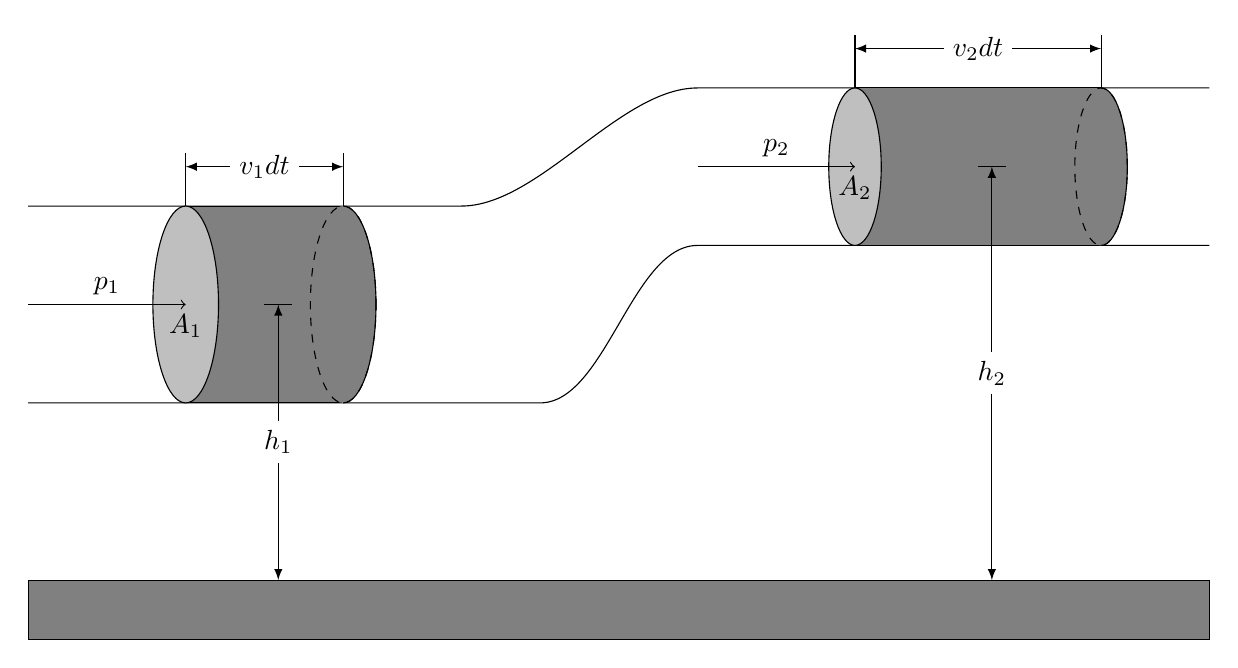
\begin{tikzpicture}
  \def\XSTART{0}
  \def\YSTART{3}
  \def\YDIAONE{2.5}
  \def\YDIATWO{2}
  \def\YCURVE{2}
  \def\XCURVE{2}
  \def\XEND{15}
  \def\XONESTART{2}
  \def\XONEDELTA{2}
  \def\DD{0.5}

  \def\YEND{\YSTART+\YCURVE+\YDIATWO}
  \def\XCURVESTART{\XEND/2-\XSTART/2-\XCURVE/2}
  \def\XCURVESTARTUP{\XEND/2-\XSTART/2-\XCURVE}
  \def\XCURVEEND{\XEND/2-\XSTART/2 + \XCURVE/2}
  \def\XONEEND{\XONESTART+\XONEDELTA}
  \def\XTWOSTART{\XCURVEEND+\XONESTART}
  \def\XTWODELTA{\XONEDELTA*\YDIAONE*\YDIAONE/\YDIATWO/\YDIATWO}
  \def\XTWOEND{\XTWOSTART+\XTWODELTA}
  \def\YTWOMIDDLE{\YSTART+\YCURVE+\YDIATWO/2}
  \def\YONEMIDDLE{\YSTART+\YDIAONE/2}
  \def\GROUND{\YSTART/4}

  \tikzset{
      partial ellipse/.style args={#1:#2:#3}{
          insert path={+ (#1:#3) arc (#1:#2:#3)}
      },
      dimen/.style={<->,>=latex,thin,
        every rectangle node/.style={fill=white,midway,font=\sffamily}},
  }

  \draw (\XSTART,\YSTART) -- (\XCURVESTART,\YSTART)
    to[out=0, in=180, looseness=0.75]
      (\XCURVEEND,{\YSTART+\YCURVE}) -- (\XEND,{\YSTART+\YCURVE});
  \draw (\XSTART,{\YSTART+\YDIAONE}) -- (\XCURVESTARTUP,{\YSTART+\YDIAONE})
    to[out=0, in=180, looseness=0.75] (\XCURVEEND,\YEND) -- (\XEND,\YEND);

  \draw [fill=gray] (\XONESTART,\YSTART) coordinate (BA)
    rectangle (\XONEEND,{\YSTART+\YDIAONE}) coordinate (BB);
  \draw [fill=lightgray](\XONESTART,\YONEMIDDLE) node [below] {$A_1$}
    ellipse ({\YDIAONE/6} and {\YDIAONE/2});
  \draw [fill=gray,dashed](\XONEEND,\YONEMIDDLE)
    ellipse ({\YDIAONE/6} and {\YDIAONE/2});
  \draw (\XONEEND,\YONEMIDDLE)
    [partial ellipse=-90:90:{\YDIAONE/6} and {\YDIAONE/2}];

  \draw [fill=gray] (\XTWOSTART,{\YSTART+\YCURVE}) coordinate (CA)
    rectangle (\XTWOEND,{\YSTART+\YCURVE+\YDIATWO}) coordinate (CB);
  \draw [fill=lightgray] (\XTWOSTART,\YTWOMIDDLE) node [below] {$A_2$}
    ellipse ({\YDIATWO/6} and {\YDIATWO/2});
  \draw [fill=gray,dashed](\XTWOEND,\YTWOMIDDLE)
    ellipse ({\YDIATWO/6} and {\YDIATWO/2});
  \draw (\XTWOEND,{\YSTART+\YCURVE+\YDIATWO/2})
    [partial ellipse=-90:90:{\YDIATWO/6} and {\YDIATWO/2}];

  \draw [fill=gray] (0,0) rectangle  (\XEND,\GROUND);

  \draw ($(BA)+(0,\YDIAONE)$) -- ++(0,\DD) coordinate (D1) -- +(0,5pt);
  \draw (BB) -- ++(0,\DD) coordinate (D2) -- +(0,5pt);
  \draw [dimen] (D1) -- (D2) node {$v_1dt$};

  \draw ($(BA)!0.5!(BB)$) -- ++(5pt,0) coordinate (E) -- +(5pt,0);
  \draw [dimen] let \p{E}=(E) in (\x{E},\GROUND) -- (E) node {$h_1$};
  \draw [style=->](\XSTART,\YONEMIDDLE) -- (\XONESTART,\YONEMIDDLE)
    node [midway,above] {$p_1$};


  \draw ($(CA)+(0,\YDIATWO)$) -- ++(0,\DD) coordinate (D1) -- +(0,5pt);
  \draw (CB) -- ++(0,\DD) coordinate (D2) -- +(0,5pt);
  \draw [dimen] (D1) -- (D2) node {$v_2dt$};

  \draw ($(CA)!0.5!(CB)$) -- ++(5pt,0) coordinate (D) -- +(5pt,0);
  \draw [dimen] let \p{D}=(D) in (\x{D},\GROUND) -- (D) node {$h_2$};
  \draw [style=->](\XCURVEEND,\YTWOMIDDLE) -- (\XTWOSTART,\YTWOMIDDLE)
    node [midway,above] {$p_2$};
\end{tikzpicture}
\end{document}